\documentclass[10pt,journal,compsoc]{IEEEtran}
\usepackage[T1]{fontenc}
\usepackage{amsmath}
\usepackage{graphicx}
\usepackage{booktabs}
\usepackage{array}
\usepackage{url}
\usepackage[nocompress]{cite}
\usepackage{tikz}
\usetikzlibrary{arrows.meta,positioning,fit,calc}

\begin{document}

\title{CS 550 Project Status Report:\\Replication of the Hawkeye and
Mockingjay Cache Replacement Policies}

\author{Vito Wang, Endong Dai, and Xiaotian Tong}

\IEEEtitleabstractindextext{%
\begin{abstract}
This report describes our progress in replicating two cache replacement
policies that learn from Belady's optimal algorithm, Hawkeye and Mockingjay, in
gem5. Hawkeye is implemented, validated against a reference model, and
evaluated on six SPEC CPU2017 benchmarks and three last-level cache (LLC)
sizes. It reduces LLC misses by 6.3\% on mcf, the benchmark with the most LLC
misses, but increases them on omnetpp and gcc. We traced most of this increase
to instruction lines that Hawkeye predicts are not worth keeping. A variant
that always keeps instruction lines removes most of the loss. For Mockingjay,
we built a reference model that reproduces the storage of the original design
and gives the expected results of our microbenchmarks. Its gem5 implementation
is behind schedule, and we give a revised timeline.
\end{abstract}

\begin{IEEEkeywords}
Cache replacement, last-level cache, Belady's algorithm, gem5
\end{IEEEkeywords}}

\maketitle
\IEEEdisplaynontitleabstractindextext

%% ------------------------------------------------------------------
\IEEEraisesectionheading{\section{Introduction \& Problem Statement}}

\IEEEPARstart{T}{he} last-level cache (LLC) is the last on-chip structure that
can hide the long latency of DRAM, so every LLC miss stalls the processor for
hundreds of cycles. When the LLC is full, the replacement policy chooses which
line to evict, and this choice largely decides the miss rate. The common
least-recently-used (LRU) policy fails when a program cycles through a working
set larger than the cache, and when data that is never reused pushes useful
lines out. Improved policies handle some of these patterns, for example by
inserting new lines with a low priority (RRIP~\cite{rrip}) or by learning which
load instructions bring in lines that are reused (SHiP~\cite{ship}). However,
each is built around a particular class of access patterns.

Belady's algorithm~\cite{belady}, also called OPT, evicts the line whose next
use lies furthest in the future. It is optimal but needs future knowledge.
Hawkeye~\cite{hawkeye} computes what OPT would have done on past accesses and
learns which load instructions bring in lines that OPT would keep. Its
follow-up, Mockingjay~\cite{mockingjay}, predicts how far in the future each
line will be reused, which lets it order lines the way OPT does. Both were
evaluated in trace-driven simulators, and gem5 includes neither of them.
This project implements both policies in gem5~\cite{gem5,gem5v20}, verifies
their functional correctness, and compares their miss rate and performance with
each other and with the baseline policies in gem5.

%% ------------------------------------------------------------------
\section{Related Work}

LRU and LFU rank lines by recency or frequency~\cite{hp6}. RRIP~\cite{rrip}
predicts how soon each line will be re-referenced with a 2- or 3-bit counter per
line, and DRRIP chooses between two RRIP variants at run time through set
dueling~\cite{dip}. A previous CS 550 project evaluated these policies in gem5,
and we use them as baselines. SHiP~\cite{ship} learns for each program counter
(PC) whether the lines it inserts are reused, and SDBP~\cite{sdbp} predicts
dead blocks from a small sampler. Both learn from a heuristic policy, so they
inherit its limits. Hawkeye~\cite{hawkeye} and Mockingjay~\cite{mockingjay}
instead learn from OPT itself. Hawkeye won the 2nd Cache Replacement
Championship (CRC2)~\cite{crc2}. We use its CRC2 code and a public ChampSim
implementation of Mockingjay as references.

%% ------------------------------------------------------------------
\section{Research Questions}

\begin{itemize}
\item \textbf{What are the Hawkeye and Mockingjay policies, and can they be
implemented correctly in gem5?}
\item \textbf{How do their LLC miss rate and IPC compare with each other and
with LRU, DRRIP, and SHiP?}
\item \textbf{Why can they reduce misses where LRU and RRIP fail, and when does
predicting reuse distances help more than a keep-or-evict decision?}
\end{itemize}

%% ------------------------------------------------------------------
\section{Hypothesis \& Proposed Solution}

We hypothesize that learning from OPT lets both policies reduce LLC misses on
access patterns where LRU and RRIP fail, such as a working set slightly larger
than the cache, or reused data mixed with data that is used only once. We also
expect Mockingjay to do better than Hawkeye when lines are reused at different
but predictable distances, because it can tell which of the lines worth keeping
will be reused last. Fig.~\ref{fig:arch} shows where both policies sit in our
gem5 system and their structures.

\begin{figure*}[t]
\centering
\resizebox{\textwidth}{!}{%
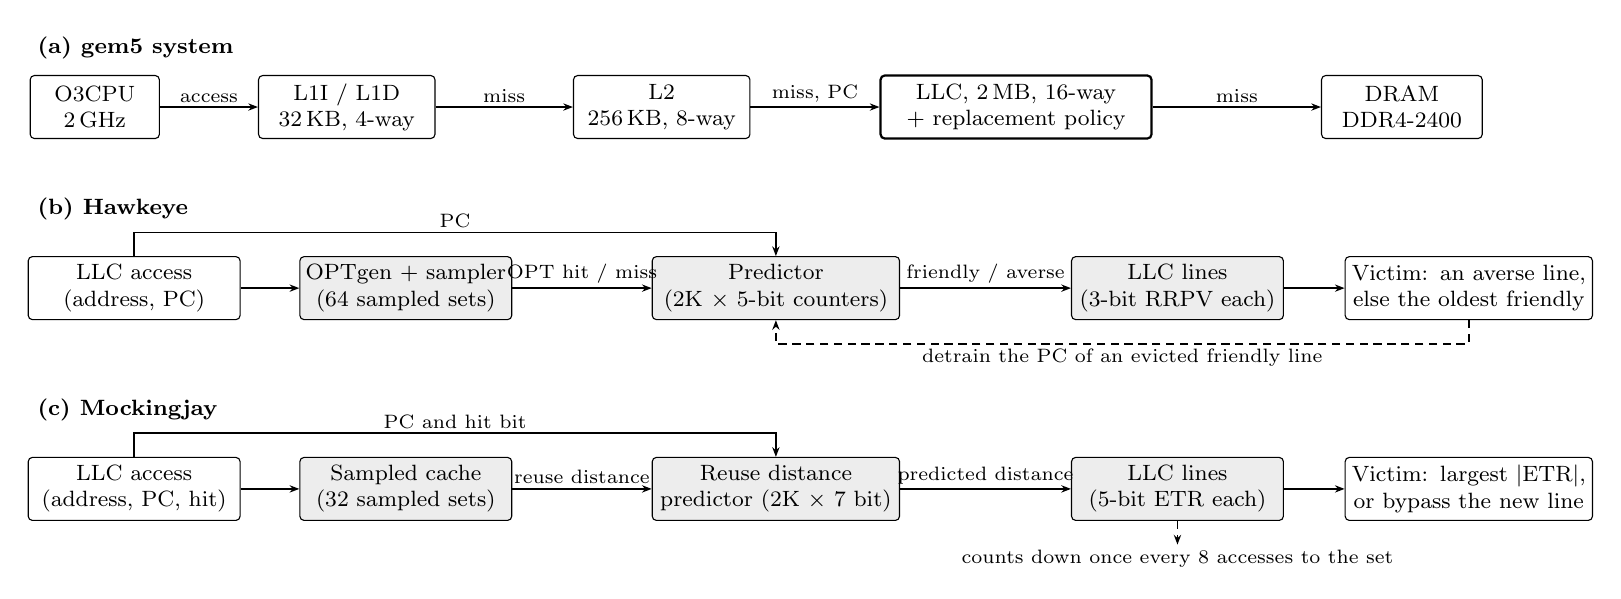
\begin{tikzpicture}[font=\footnotesize,
  box/.style={draw, rounded corners=1.5pt, align=center, inner sep=2pt,
              minimum height=0.8cm, text width=2.55cm},
  st/.style={box, fill=black!7},
  arr/.style={-{Stealth[length=3.5pt]}, semithick},
  lab/.style={font=\scriptsize, inner sep=1.5pt},
  row/.style={font=\footnotesize\bfseries, anchor=west}]
% columns shared by rows (b) and (c)
\def\ca{1.3}\def\cb{4.75}\def\cc{9.45}\def\cd{14.55}\def\ce{18.25}
% (a) the gem5 system
\node[row] at (-0.05,0.75) {(a) gem5 system};
\node[box, text width=1.5cm] (cpu) at (0.8,0) {O3CPU\\2\,GHz};
\node[box, text width=2.1cm] (l1) at (4.0,0) {L1I / L1D\\32\,KB, 4-way};
\node[box, text width=2.1cm] (l2) at (8.0,0) {L2\\256\,KB, 8-way};
\node[box, text width=3.3cm, thick] (llc) at (12.5,0)
  {LLC, 2\,MB, 16-way\\+ replacement policy};
\node[box, text width=1.9cm] (dram) at (17.4,0) {DRAM\\DDR4-2400};
\draw[arr] (cpu) -- node[lab, above] {access} (l1);
\draw[arr] (l1) -- node[lab, above] {miss} (l2);
\draw[arr] (l2) -- node[lab, above] {miss, PC} (llc);
\draw[arr] (llc) -- node[lab, above] {miss} (dram);
% (b) Hawkeye
\begin{scope}[yshift=-2.3cm]
\node[row] at (-0.05,1.0) {(b) Hawkeye};
\node[box] (ha) at (\ca,0) {LLC access\\(address, PC)};
\node[st] (og) at (\cb,0) {OPTgen + sampler\\(64 sampled sets)};
\node[st, text width=3.0cm] (hp) at (\cc,0) {Predictor\\(2K $\times$ 5-bit counters)};
\node[st] (rr) at (\cd,0) {LLC lines\\(3-bit RRPV each)};
\node[box, text width=3.0cm] (hv) at (\ce,0) {Victim: an averse line,\\else the oldest friendly};
\draw[arr] (ha) -- (og);
\draw[arr] (og) -- node[lab, above] {OPT hit / miss} (hp);
\draw[arr] (hp) -- node[lab, above] {friendly / averse} (rr);
\draw[arr] (rr) -- (hv);
\draw[arr] (ha.north) -- ++(0,0.3) -| node[lab, pos=0.25, above] {PC} (hp.north);
\draw[arr, densely dashed] (hv.south) -- ++(0,-0.3) -| node[lab, pos=0.25, below]
  {detrain the PC of an evicted friendly line} (hp.south);
\end{scope}
% (c) Mockingjay
\begin{scope}[yshift=-4.85cm]
\node[row] at (-0.05,1.0) {(c) Mockingjay};
\node[box] (ma) at (\ca,0) {LLC access\\(address, PC, hit)};
\node[st] (sc) at (\cb,0) {Sampled cache\\(32 sampled sets)};
\node[st, text width=3.0cm] (rdp) at (\cc,0) {Reuse distance\\predictor (2K $\times$ 7 bit)};
\node[st] (etr) at (\cd,0) {LLC lines\\(5-bit ETR each)};
\node[box, text width=3.0cm] (mv) at (\ce,0) {Victim: largest $|$ETR$|$,\\or bypass the new line};
\draw[arr] (ma) -- (sc);
\draw[arr] (sc) -- node[lab, above] {reuse distance} (rdp);
\draw[arr] (rdp) -- node[lab, above] {predicted distance} (etr);
\draw[arr] (etr) -- (mv);
\draw[arr] (ma.north) -- ++(0,0.3) -| node[lab, pos=0.25, above] {PC and hit bit} (rdp.north);
\draw[arr, densely dashed] (etr.south) -- ++(0,-0.3) node[lab, below]
  {counts down once every 8 accesses to the set};
\end{scope}
\end{tikzpicture}}
\caption{(a) The gem5 system. The PC travels with each request to the LLC.
(b) Hawkeye and (c) Mockingjay. Shaded boxes are the structures that each
policy adds, with sizes for a 2\,MB LLC.}
\label{fig:arch}
\end{figure*}

\subsection{Hawkeye}

\textbf{OPTgen} reconstructs OPT's decisions on a sample of 64 sets. When a
line is accessed again, it checks whether OPT could have kept the line since its
previous access without exceeding the cache capacity. A \textbf{sampler}
remembers the PC that last accessed each line of these sets. The
\textbf{predictor} keeps a 5-bit counter for each hashed PC. It counts up when
OPT would have hit and down when OPT would have missed. A line whose PC counter
is in the upper half is \emph{cache-friendly} and is inserted with a 3-bit
re-reference prediction value (RRPV) of 0. Otherwise it is
\emph{cache-averse} and inserted with RRPV 7. Hawkeye evicts an averse line
first. If there is none, it evicts the oldest friendly line and, if the line is
in a sampled set, lowers the counter of the PC that brought it in.

\subsection{Mockingjay}

The \textbf{sampled cache} records recent accesses to 32 sampled sets. When a
line is accessed again, it measures the reuse distance, i.e., the number of
accesses to the set since the previous access. A line that is not reused
within 127 accesses is treated as never reused. The \textbf{reuse distance
predictor (RDP)} learns the typical reuse distance of the lines brought in by
each PC. Each LLC line keeps a 5-bit \textbf{estimated time remaining (ETR)}.
It starts at the predicted reuse distance divided by 8 and counts down once
every 8 accesses to the set. Mockingjay evicts the line with the largest
$|$ETR$|$, which is either reused furthest in the future or most overdue. If the
incoming line would be reused later than every line in the set, Mockingjay does
not insert it.

%% ------------------------------------------------------------------
\section{Evaluation}

\begin{figure*}[t]
\centering
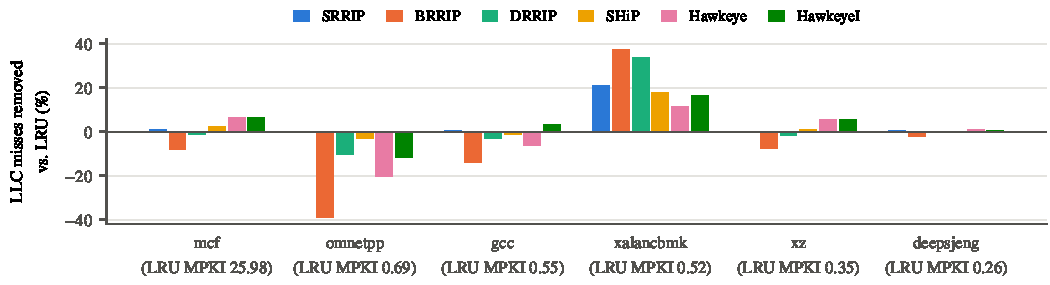
\includegraphics[width=\textwidth]{fig/spec_2mb.pdf}
\caption{LLC misses removed relative to LRU with a 2\,MB LLC. Benchmarks are
sorted by the LRU miss rate. HawkeyeI always keeps instruction lines.}
\label{fig:spec}
\end{figure*}

\subsection{Methodology}

We use gem5 v23.0.0.1 in syscall-emulation mode with the x86 out-of-order CPU
model (O3CPU) and the cache hierarchy of Fig.~\ref{fig:arch}(a), without
hardware prefetching. For SPEC CPU2017~\cite{spec17}, an atomic CPU skips the
first one billion instructions, and the O3CPU then runs 50 million instructions
of warmup and 200 million measured instructions. We use the speed versions of
mcf, omnetpp, and xalancbmk, and the rate versions of gcc, xz, and deepsjeng,
because the speed versions of these three need 7 to 15\,GB of memory and the
course instance has 15\,GB.

\emph{Progress made.} We added the LLC and the fast-forward step to the course
configuration. Hawkeye is a new class (630 lines of C++) in gem5's
replacement-policy interface, with a debug flag and statistics. While
validating it, we found and fixed three gem5 problems that affect any PC-based
policy. First, the L2 notifies the LLC of every clean eviction, and gem5 passes
these notifications to the replacement policy as if they were accesses. Hawkeye
trained on 8.7 million of them in mcf, so it now ignores them. Second, gem5's
x86-64 \texttt{newfstatat} system call used the wrong file-status structure, so
omnetpp and gcc failed to start. Third, gem5 dropped the PC when the L1
forwarded a software prefetch, so 28\% of omnetpp's LLC accesses had no PC.

For Mockingjay, we mapped the original design onto gem5's interface. gem5's
policies cannot refuse an insertion. However, a line that Mockingjay would not
insert gets an ETR larger than every other line in the set, so inserting it
normally makes it the next victim. Also, gem5 passes only the accessed line to
the policy, so the policy cannot age the whole set every 8 accesses. Each line
instead records the set's aging count when its ETR is set, and the current ETR
is computed when the line is compared.

\subsection{Functional Validation}

\emph{Progress made.} We validate each policy with logs and with
microbenchmarks. The Hawkeye debug flag prints every OPTgen decision,
prediction, and victim. A Python reference model replays the logged LLC
accesses through its own OPTgen and compares every decision. It also prints a
short example that can be checked by hand. On a 345,074-access log, gem5 and the
model made the same 9,218 OPTgen decisions with no mismatch.

\begin{table}[t]
\centering
\caption{LLC miss rate (\%) on the microbenchmarks}
\label{tab:micro}
\setlength{\tabcolsep}{5pt}
\begin{tabular}{@{}llrrr@{}}
\toprule
& Policy & fit & thrash & mix \\
\midrule
gem5, 6 passes & LRU, SRRIP & 15.0 & 100 & 100 \\
& BRRIP & 15.0 & 46.8 & 96.4 \\
& DRRIP & 15.0 & 61.7 & 99.1 \\
& SHiP & 15.0 & 90.0 & 100 \\
& Hawkeye & 15.0 & 48.1 & 88.3 \\
\midrule
Model, 6 passes & OPT & 14.3 & 42.9 & 87.3 \\
& Mockingjay & 14.3 & 54.2 & 96.4 \\
& \quad no bypass & 14.3 & 55.4 & 96.4 \\
\midrule
Model, 20 passes & OPT & 4.8 & 36.5 & 88.4 \\
& Mockingjay & 4.8 & 41.3 & 91.2 \\
& \quad no bypass & 4.8 & 41.7 & 91.2 \\
\bottomrule
\end{tabular}
\end{table}

Table~\ref{tab:micro} shows our three microbenchmarks. \emph{fit} loops over a
1\,MB array, \emph{thrash} over a 3\,MB array, and \emph{mix} alternates a
1\,MB reused array with a stream that is never reused. All policies behave as
expected. In fit, every policy has only compulsory misses. In thrash, LRU
misses on every access, while Hawkeye keeps part of the array, as BRRIP does.
In mix, only Hawkeye separates the reused array from the stream. For each
microbenchmark, the program output is identical under all six policies.

For Mockingjay, we wrote a second reference model that follows the public
ChampSim code. It replays the same LLC accesses as our microbenchmarks. The OPT miss rate
of these streams (42.9\% on thrash) matches the 43.0\% that we computed from
the gem5 log, so they model the gem5 runs closely. These results are the
expected values for the gem5 implementation. They also show two things for our
plan. First, the lack of bypass in gem5 costs at most 1.2 points. Second,
Mockingjay learns slowly on short runs. It decides that a line is not reused
only after 127 accesses to its set, so on mix it starts keeping the reused array only
in the fourth pass. We will therefore run its microbenchmarks for 20 passes.
Finally, the model runs the original aging and our gem5 version side by side,
and they made the same decision on all 1.36 million accesses.

\subsection{Physical Characteristics}

We do not implement Verilog, so we estimate the hardware cost from the
storage of the added structures. For a 2\,MB LLC, our Hawkeye needs 30.0\,KB
and the paper reports 28\,KB. The difference comes from the parameters of the
CRC2 code that we follow. For example, its OPTgen records every access instead
of every fourth access. Our Mockingjay model needs
31.91\,KB, the same as the paper. Both fit in the 32\,KB budget of CRC2.

\subsection{Performance Impact}



\emph{Results so far.} Fig.~\ref{fig:spec} compares the policies with a 2\,MB
LLC. On mcf, which has 38 times the LLC misses per kilo-instruction (MPKI)
of any other benchmark, Hawkeye removes 6.3\% of the misses and improves IPC
by 1.4\%. No built-in policy improves IPC by more than 0.1\%. On xalancbmk,
Hawkeye removes 11.5\% of the misses, fewer than every built-in policy, while
BRRIP removes 37.4\%. On omnetpp and gcc,
Hawkeye increases misses by 20.4\% and 6.2\%.

To explain these losses, we added statistics that separate instruction and data
lines. In gem5, the PC of an instruction fetch is the fetch address itself, so
every instruction line has its own entry in the predictor. On omnetpp,
Hawkeye predicted 14\% of the instruction fetches as cache-averse, and its LLC
instruction misses rose from 662 under LRU to 11,113. On gcc, Hawkeye has fewer
data misses than LRU and loses only because of instruction misses. We tested
three changes. Refreshing a line when the L2 evicts its copy changed little.
Doing so for every line reduced the loss on omnetpp but hurt the other
benchmarks. Always inserting instruction lines as friendly (HawkeyeI) brought
instruction misses down to the level of LRU or below on every benchmark. As a result, gcc now gains
3.1\%, xalancbmk gains 16.5\%, and the loss on omnetpp drops to 11.6\%. The
remaining loss on omnetpp comes from data lines, and we are still analyzing it.

\begin{table}[t]
\centering
\caption{LLC misses removed vs.\ LRU (\%) / IPC speedup vs.\ LRU for three LLC
sizes. ``Best'' is the built-in policy with the highest IPC.}
\label{tab:sweep}
\setlength{\tabcolsep}{3.2pt}
\begin{tabular}{@{}llrrr@{}}
\toprule
& LLC & Best baseline & Hawkeye & HawkeyeI \\
\midrule
mcf & 1\,MB & SHiP $+$7.8 / 1.012 & $+$6.3 / 1.016 & $+$6.3 / 1.016 \\
& 2\,MB & SRRIP $+$1.0 / 1.000 & $+$6.3 / 1.014 & $+$6.3 / 1.014 \\
& 4\,MB & SRRIP $+$2.7 / 1.015 & $+$10.8 / 1.076 & $+$10.8 / 1.076 \\
\midrule
xalanc. & 1\,MB & BRRIP $+$52.8 / 1.213 & $+$19.5 / 1.061 & $+$22.6 / 1.075 \\
& 2\,MB & BRRIP $+$37.4 / 1.023 & $+$11.5 / 1.006 & $+$16.5 / 1.009 \\
& 4\,MB & DRRIP $+$2.2 / 1.000 & $+$1.3 / 1.000 & $+$4.5 / 1.001 \\
\midrule
omnetpp & 1\,MB & SHiP $-$15.5 / 1.000 & $-$12.8 / 0.988 & $-$4.1 / 0.995 \\
& 2\,MB & SHiP $-$3.0 / 1.000 & $-$20.4 / 0.986 & $-$11.6 / 0.991 \\
& 4\,MB & SHiP $-$0.2 / 0.997 & $-$9.9 / 0.989 & $-$5.6 / 0.991 \\
\bottomrule
\end{tabular}
\end{table}

Table~\ref{tab:sweep} repeats the comparison for 1\,MB and 4\,MB LLCs. On mcf,
Hawkeye has the highest IPC at every size, and its advantage grows with the
LLC. With 4\,MB it removes 10.8\% of the misses and improves IPC by 7.6\%. On
xalancbmk, the working set is between 1\,MB and 4\,MB, and BRRIP stays well
ahead of Hawkeye at 1\,MB and 2\,MB. Most of this gap comes from data lines, so
HawkeyeI closes only a small part of it. On omnetpp, no policy has fewer misses
than LRU, and
instruction lines cause 71\%, 37\%, and 34\% of Hawkeye's extra misses at the
three sizes. HawkeyeI improves IPC over Hawkeye on xalancbmk and omnetpp at
every size.

%% ------------------------------------------------------------------
\section{Milestones}

\begin{table}[t]
\centering
\caption{Milestone status as of Nov.~11}
\label{tab:milestones}
\setlength{\tabcolsep}{3pt}
\begin{tabular}{@{}>{\raggedright}p{0.36\columnwidth}>{\raggedright\arraybackslash}p{0.58\columnwidth}@{}}
\toprule
Milestone (planned week) & Status \\
\midrule
1. Setup (Week 1, Oct.~29--Nov.~4) & Completed. \\
2. Implementation (Week 2, Nov.~5--11) & Hawkeye completed in Week 1. Mockingjay design and reference model completed, gem5 code behind (new date Nov.~18). \\
3. Functional validation (Week 3, Nov.~12--18) & Hawkeye completed early. Mockingjay expected values ready, gem5 runs by Nov.~22. \\
4. Performance evaluation (Week 4, Nov.~19--25) & Hawkeye completed early, with all three LLC sizes. Mockingjay by Nov.~26. \\
5. Final report (Week 5, Nov.~26--Dec.~3) & Not started, on schedule. \\
\bottomrule
\end{tabular}
\end{table}

Table~\ref{tab:milestones} lists our milestones. Milestone~1 is complete. The
LLC, the O3CPU, and the baseline policies run in gem5, and every demand access
to the LLC carries a PC. The Hawkeye parts of Milestones~2 to 4 are complete two to three
weeks ahead of the plan. Beyond the plan, we also found and fixed three gem5
problems, explained Hawkeye's losses, and tested three variants of it.

We have not met Milestone~2 for Mockingjay. We added Mockingjay on Nov.~2,
after the feedback on our proposal, so its work started a week later than
Hawkeye's. We also chose to finish the Hawkeye evaluation first, because its
analysis exposed gem5 issues that Mockingjay must also handle, i.e., clean
eviction notices, missing PCs, and instruction fetches. So far, we have mapped
Mockingjay onto gem5's interface and built and checked its reference model.
Mockingjay reuses the LLC configuration, scripts, microbenchmarks, and
validation flow of Hawkeye, so we plan to complete its gem5 code by Nov.~18,
validate it by Nov.~22, and finish its SPEC runs at all three LLC sizes by
Nov.~26. This keeps the final report on schedule.

%% ------------------------------------------------------------------
\section{Division of Labor}

Each of us delivers part of the gem5 code. Vito and Endong work on Hawkeye,
including its implementation in gem5 and the microbenchmarks for its functional
validation. Vito and Xiaotian do the same for Mockingjay. Endong and Xiaotian
run the baseline and SPEC CPU2017 simulations, repeat them for the other LLC
sizes, and collect and plot the statistics. All three analyze the results and
write the final report.

%% ------------------------------------------------------------------
\begin{thebibliography}{99}

\bibitem{rrip}
A. Jaleel, K. B. Theobald, S. C. Steely Jr., and J. Emer, ``High performance
cache replacement using re-reference interval prediction (RRIP),'' in
\emph{Proc. ISCA}, 2010.

\bibitem{ship}
C.-J. Wu, A. Jaleel, W. Hasenplaugh, M. Martonosi, S. C. Steely Jr., and
J. Emer, ``SHiP: Signature-based hit predictor for high performance caching,''
in \emph{Proc. MICRO}, 2011.

\bibitem{belady}
L. A. Belady, ``A study of replacement algorithms for a virtual-storage
computer,'' \emph{IBM Systems Journal}, vol. 5, no. 2, pp. 78--101, 1966.

\bibitem{hawkeye}
A. Jain and C. Lin, ``Back to the future: Leveraging Belady's algorithm for
improved cache replacement,'' in \emph{Proc. ISCA}, 2016.

\bibitem{mockingjay}
I. Shah, A. Jain, and C. Lin, ``Effective mimicry of Belady's MIN policy,'' in
\emph{Proc. HPCA}, 2022.

\bibitem{gem5}
N. Binkert \emph{et al.}, ``The gem5 simulator,'' \emph{ACM SIGARCH Comput.
Archit. News}, vol. 39, no. 2, pp. 1--7, 2011.

\bibitem{gem5v20}
J. Lowe-Power \emph{et al.}, ``The gem5 simulator: Version 20.0+,''
arXiv:2007.03152, 2020.

\bibitem{hp6}
J. L. Hennessy and D. A. Patterson, \emph{Computer Architecture: A Quantitative
Approach}, 6th ed. Morgan Kaufmann, 2019.

\bibitem{dip}
M. K. Qureshi, A. Jaleel, Y. N. Patt, S. C. Steely Jr., and J. Emer, ``Adaptive
insertion policies for high performance caching,'' in \emph{Proc. ISCA}, 2007.

\bibitem{sdbp}
S. M. Khan, Y. Tian, and D. A. Jim\'enez, ``Sampling dead block prediction for
last-level caches,'' in \emph{Proc. MICRO}, 2010.

\bibitem{crc2}
The 2nd Cache Replacement Championship (CRC2), held with ISCA 2017.

\bibitem{spec17}
Standard Performance Evaluation Corporation, ``SPEC CPU2017,''
\url{https://www.spec.org/cpu2017/}.

\end{thebibliography}

\end{document}
